\documentclass[12pt]{article}
\usepackage[utf8]{inputenc}
\usepackage{verbatim}
\usepackage{caption}
\usepackage{float}
\usepackage{geometry}
\usepackage{graphicx}

\begin{document}

\section{Description}

Optical Jigsaw outreach demo, used to demonstrate guiding light using differences in refractive indices and repeaters.


\section{Introduction - Adults}

Transmitting information using light forms the basis of nearly all modern communications, including the internet. This demo is a small scale (toy) copy of the things you need to talk to someone so far away that it would take you 10 hours to travel there but you can have a conversation with them in real time! 

We are using light to send our message, light is a great carrier of information as it is the fastest thing in the universe. Most of the world uses fibre optic cables which are under water on the ocean floor. Fibre optic cables are made of glass which is close to the width of a human hair.

In our demo we are using a type of plastic (perspex) which has very similar properties but on a much larger scale. We use lightpipes to guide light around, similarly to how water flows through pipes. The proper name for them are waveguides, but lightpipes sounds more fun! The light is contained inside the optical fibre or lightpipe due to total internal reflection.

\begin{figure}[h]
\centering
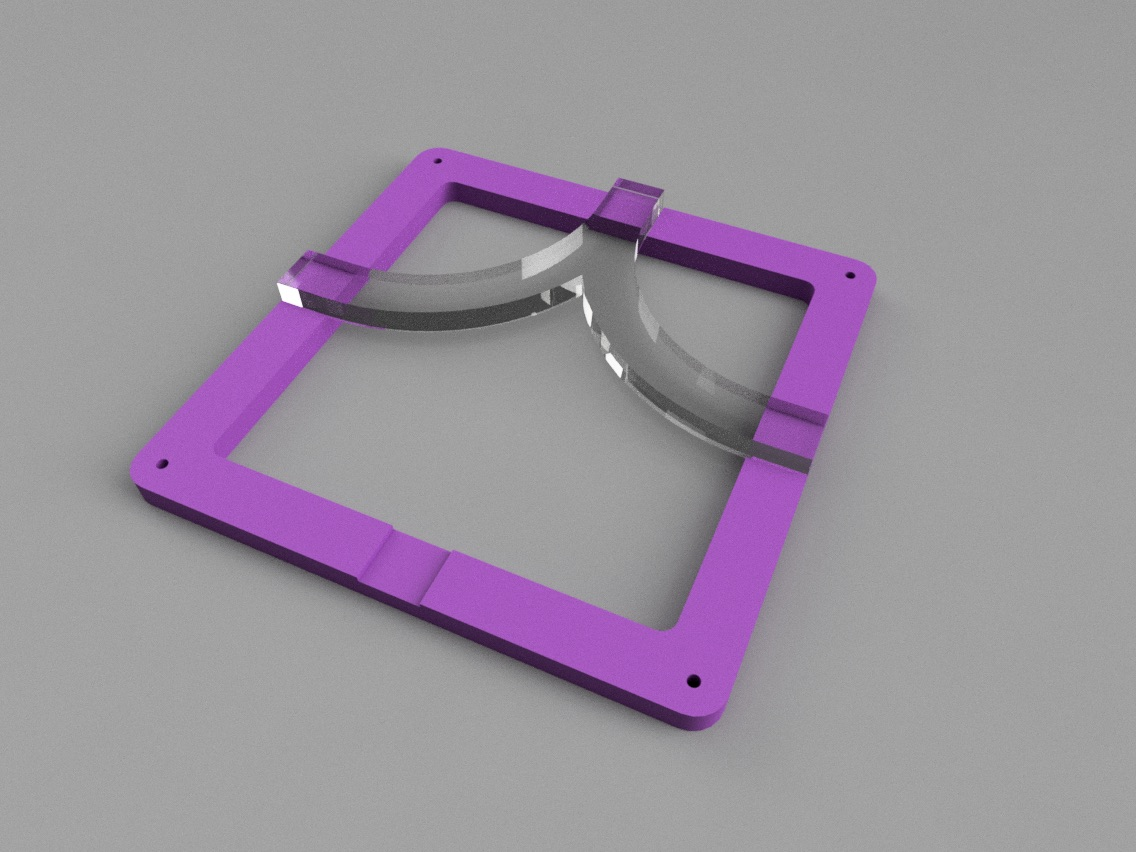
\includegraphics[width=0.45\textwidth]{figures/jigsaw_y-junction.jpg}
\caption{Splitter}
\end{figure}

You can do some pretty nice things using lightpipes. There are straight and curved sections, and we can also split the light into two paths. In fact the lightpipes here are bigger versions of some of the components that make up a quantum computer. A quantum computer is a new type of computer which will be able to solve problems no other computer can.

The problem with guiding light is that the light leaks out of the lightpipes. You can see this as the lightpipes get dimmer after each block. We use a repeater to make the light brighter.  

The object of the demo is to get light from one end to the other using the lightpipe blocks.

\section{User instructions}

\begin{itemize}
    \item The rechargeable torches (micro-usb) work best as sources, there are a few torch holder
        frames which, using fishing wire or string can be used to hold the torches.
    \item Batteries, each repeater lasts between 6-10 hours on a single 9V battery, there
        is an on-off switch for each repeater board.
    \item Due to an issue with back-reflection causing the repeaters to trigger
        themselves in both directions we have taken out the LDRs on one side of each of
        the repeaters meaning they are now only one-directional.
    \item Each LED on the repeaters has a POT (potentiometer) associated to it, tuning
        the POT tunes the sensitivity to incoming light, there are arrows next to each
        POT which point to the LED it tunes.
    \item The demo works best in dark or constant light-level rooms, otherwise frequent
        tuning is needed to ensure the LEDs trigger properly.
    \item We found that each repeater worked for around 3 blocks, the corner pieces and
        crossers are very lossy.
\end{itemize}


\section{Troubleshooting}

\textbf{If a repeater isn't working,}
\begin{enumerate}
\item Check the switch is on
\item Check it is facing in the correct direction, the LDR should be on the side with
\item Reduce the number of lightpipes between the repeater ad the source.
    incoming light.
\item Try tuning the POT to the maximums of both directions until the LED turns on
\item Check the batteries 
\end{enumerate}
%
\textbf{If a torch isn't working,}
\begin{enumerate}
    \item Check the torch is on, button is on the bottom of the torch
    \item Try plugging in the torch as the battery is probably flat.
\end{enumerate}


\newpage
\section{Improvements to be made}

\begin{itemize}
	\item Fix back reflection triggering a permanent loop using a microcontroller.
	\item Redesign the repeaters to work in all four directions on the square enabling 90 \degree turns 
	\item Reconfigurable directions
	\item Button to autotune background light level
	\item PWM magic
	\item Mains power supply 
	\item Colour filters
	\item Change voltage regulator/supply
	\item Wireless support
	\item Pots for current control giving adjustable brightness/power consumption	
\end{itemize}

\begin{itemize}
	\item allpcb 10 100x100mm pcbs 2mm thickness \$75.
	\item Perspex for 1000x1000mmx2mm £40
        \item Possible chip: PIC18F1230
\end{itemize}

In order to produce a DXF autocad schematic we will use FREECAD which is avaliable on the ubuntu repository.

We want to have around 15mm thickness in the perspex waveguides and they should fit on 150x150mm$^2$ blocks

Box outline with waveguides inside, 
\begin{verbatim}
---------------
|             |
|_____________|
|_____________| 
|             |
|             |
---------------

---------------
|     |  |    |
|     |  |    |
|     |  |    | 
|     |  |    |
|     |  |    |
---------------

\end{verbatim}


We want to be able to tile the squares together to create a maze. We are also including curved sections (not shown here).



\end{document}
